\section{MotorController}


\subsection{Mechanical setup}


\subsection{Electrical setup}
Instead of breadbord and a lot of lose wires a special wiring harnass was designed. 
This harnass is split into two sections, one for the three front sensors and one for the five back sensors.
The sections meet in the middle and connect to the arduino Uno.
The sections contain the common power wires, the common trigger wire and indivdual echo wires.
The wires are made from flat cable and provided with connectors which improves repair or reorientation if needed.

The wiring for the sonars can be found in the schematic below (reused from previous group):

\begin{figure}[H]
\centering
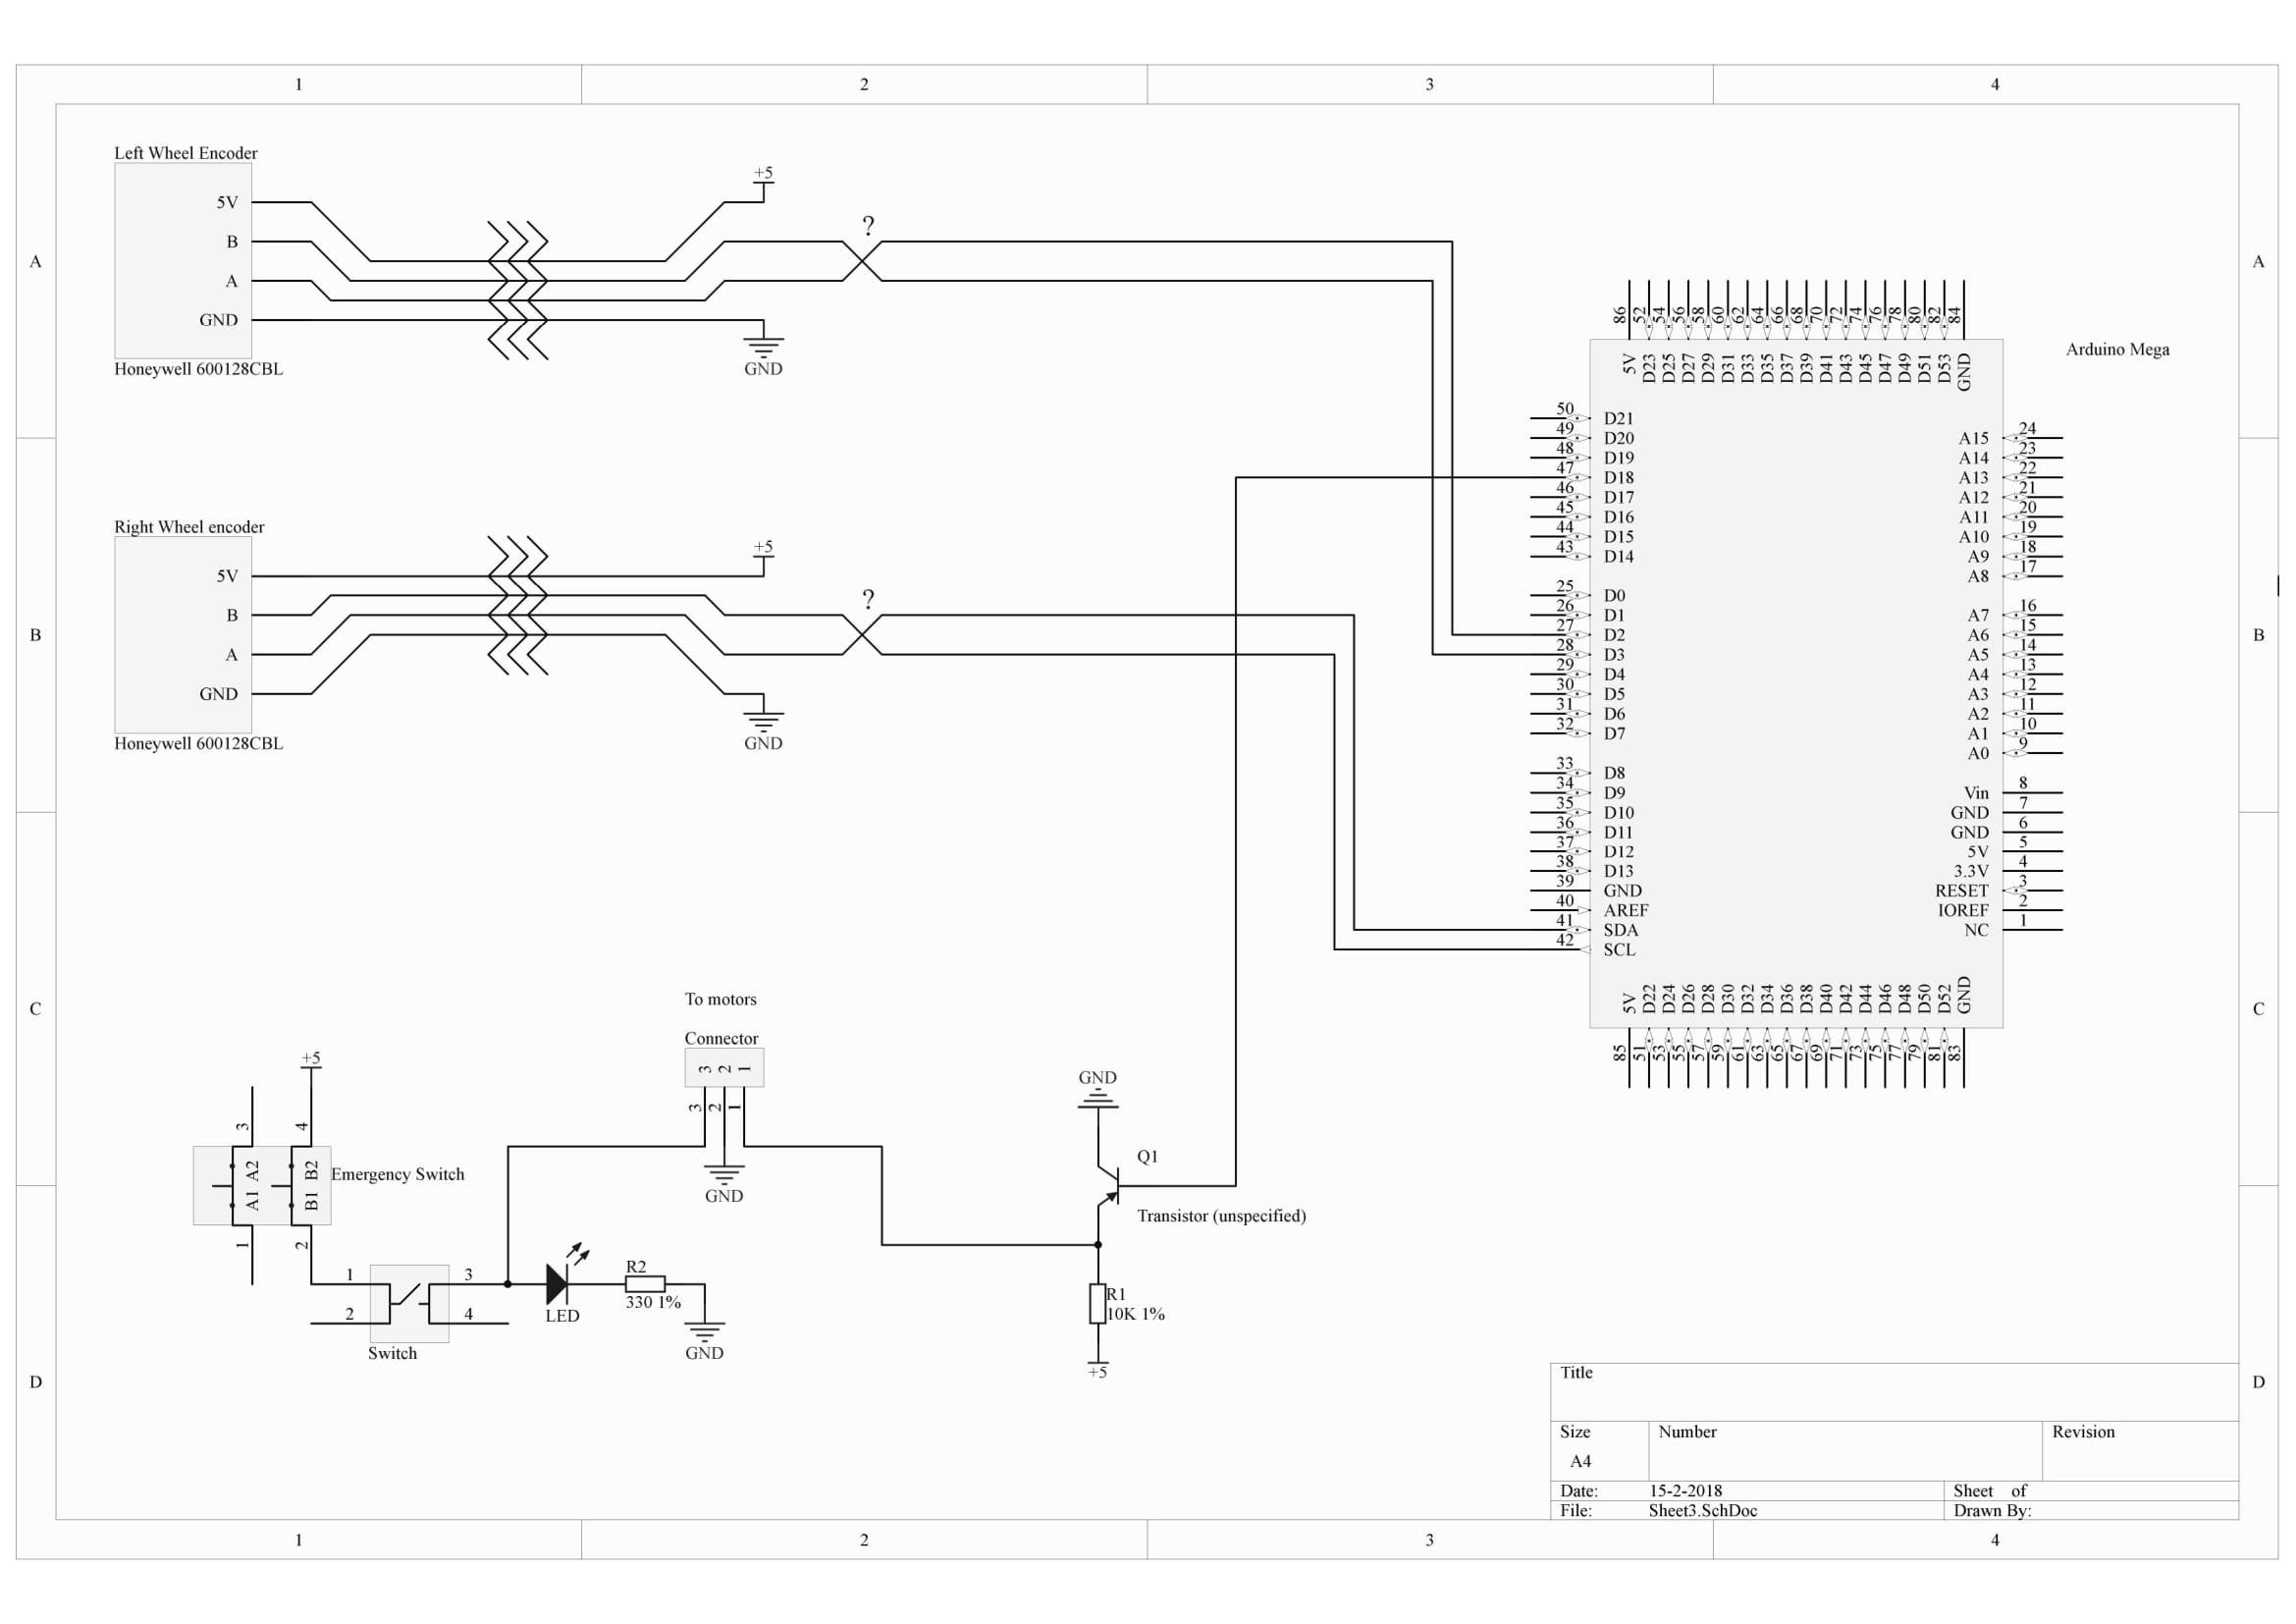
\includegraphics[width=12cm]{MotorController.jpg}
\caption{Wiring setup for the motor controller}
\label{fig::wiringMotor}
\end{figure}

 
    